\documentclass[]{book}
\usepackage{lmodern}
\usepackage{amssymb,amsmath}
\usepackage{ifxetex,ifluatex}
\usepackage{fixltx2e} % provides \textsubscript
\ifnum 0\ifxetex 1\fi\ifluatex 1\fi=0 % if pdftex
  \usepackage[T1]{fontenc}
  \usepackage[utf8]{inputenc}
\else % if luatex or xelatex
  \ifxetex
    \usepackage{mathspec}
  \else
    \usepackage{fontspec}
  \fi
  \defaultfontfeatures{Ligatures=TeX,Scale=MatchLowercase}
    \setmainfont[]{NanumGothic}
\fi
% use upquote if available, for straight quotes in verbatim environments
\IfFileExists{upquote.sty}{\usepackage{upquote}}{}
% use microtype if available
\IfFileExists{microtype.sty}{%
\usepackage{microtype}
\UseMicrotypeSet[protrusion]{basicmath} % disable protrusion for tt fonts
}{}
\usepackage[margin=1in]{geometry}
\usepackage{hyperref}
\hypersetup{unicode=true,
            pdftitle={삽화성편두통 예방 진료지침},
            pdfauthor={대한두통학회 편두통진료지침위원회},
            pdfborder={0 0 0},
            breaklinks=true}
\urlstyle{same}  % don't use monospace font for urls
\usepackage{natbib}
\bibliographystyle{apalike}
\usepackage{longtable,booktabs}
\usepackage{graphicx,grffile}
\makeatletter
\def\maxwidth{\ifdim\Gin@nat@width>\linewidth\linewidth\else\Gin@nat@width\fi}
\def\maxheight{\ifdim\Gin@nat@height>\textheight\textheight\else\Gin@nat@height\fi}
\makeatother
% Scale images if necessary, so that they will not overflow the page
% margins by default, and it is still possible to overwrite the defaults
% using explicit options in \includegraphics[width, height, ...]{}
\setkeys{Gin}{width=\maxwidth,height=\maxheight,keepaspectratio}
\IfFileExists{parskip.sty}{%
\usepackage{parskip}
}{% else
\setlength{\parindent}{0pt}
\setlength{\parskip}{6pt plus 2pt minus 1pt}
}
\setlength{\emergencystretch}{3em}  % prevent overfull lines
\providecommand{\tightlist}{%
  \setlength{\itemsep}{0pt}\setlength{\parskip}{0pt}}
\setcounter{secnumdepth}{5}
% Redefines (sub)paragraphs to behave more like sections
\ifx\paragraph\undefined\else
\let\oldparagraph\paragraph
\renewcommand{\paragraph}[1]{\oldparagraph{#1}\mbox{}}
\fi
\ifx\subparagraph\undefined\else
\let\oldsubparagraph\subparagraph
\renewcommand{\subparagraph}[1]{\oldsubparagraph{#1}\mbox{}}
\fi

%%% Use protect on footnotes to avoid problems with footnotes in titles
\let\rmarkdownfootnote\footnote%
\def\footnote{\protect\rmarkdownfootnote}

%%% Change title format to be more compact
\usepackage{titling}

% Create subtitle command for use in maketitle
\providecommand{\subtitle}[1]{
  \posttitle{
    \begin{center}\large#1\end{center}
    }
}

\setlength{\droptitle}{-2em}

  \title{삽화성편두통 예방 진료지침}
    \pretitle{\vspace{\droptitle}\centering\huge}
  \posttitle{\par}
    \author{대한두통학회 편두통진료지침위원회}
    \preauthor{\centering\large\emph}
  \postauthor{\par}
      \predate{\centering\large\emph}
  \postdate{\par}
    \date{2019-06-19}

\usepackage{booktabs}
\usepackage{amsthm}
\makeatletter
\def\thm@space@setup{%
  \thm@preskip=8pt plus 2pt minus 4pt
  \thm@postskip=\thm@preskip
}
\makeatother

\begin{document}
\maketitle

{
\setcounter{tocdepth}{1}
\tableofcontents
}
\hypertarget{section}{%
\chapter{개발그룹}\label{section}}

\hypertarget{section-1}{%
\section{운영위원회}\label{section-1}}

\begin{itemize}
\tightlist
\item
  위원장: 인제대학교 정재면
\item
  간사: 중앙대학교 박광열
\end{itemize}

\hypertarget{section-2}{%
\section{자문위원회}\label{section-2}}

\begin{itemize}
\tightlist
\item
  을지대학교 김병건
\item
  연세대학교 김원주
\end{itemize}

\hypertarget{section-3}{%
\section{외부자문그룹}\label{section-3}}

\begin{itemize}
\tightlist
\item
  순천향대학교 이유경
\item
  NECA 박동아
\end{itemize}

\hypertarget{section-4}{%
\section{실무위원회및 근거평가그룹}\label{section-4}}

\begin{itemize}
\tightlist
\item
  분당제생병원 김병수
\item
  경북대학교 서종근
\item
  한림대학교 손종희
\item
  이화여자대학교 송태진
\item
  성균관대학교 이미지
\item
  성균관대학교 정필욱
\item
  NECA 최미영
\item
  전주예수병원 최윤주
\end{itemize}

\hypertarget{section-5}{%
\section{이해관계 선언}\label{section-5}}

운영위원회및 실무위원회의 모든 위원은 자문료, 연구비, 지적재산권드의 재정적 이해상충, 지적이해상충, 그리고 개인적 이해상충을 문서로 공개하였다.

\hypertarget{section-6}{%
\section{운영}\label{section-6}}

\hypertarget{section-7}{%
\subsection{합의원칙의 결정}\label{section-7}}

\begin{itemize}
\tightlist
\item
  토론
\end{itemize}

\hypertarget{section-8}{%
\subsection{저자원칙의 결정}\label{section-8}}

\begin{itemize}
\tightlist
\item
  초안:
\item
  최종보고서: 정재면
\item
  저자포함: 개발그룹전체
\end{itemize}

\hypertarget{section-9}{%
\subsection{잠재적 승인기구}\label{section-9}}

\begin{itemize}
\tightlist
\item
  대한두통학회
\item
  대한신경과학회
\end{itemize}

\hypertarget{section-10}{%
\subsection{보급전략}\label{section-10}}

\begin{itemize}
\tightlist
\item
  대한두통학회와 대한신경과학회 홈페이지 게시
\item
  대한두통학회지와 대한신경과학회지에 게재
\end{itemize}

\hypertarget{section-11}{%
\chapter{개발 계획}\label{section-11}}

\hypertarget{section-12}{%
\section{기존 진료지침 검색}\label{section-12}}

\begin{itemize}
\item
  Selection criteria

  -- From 2012 to 2016

  -- Written in English or Korean

  -- By Multi-disciplinary team

  -- Evidence-based method
\item
  9개의 진료지침 검토

  -- 2012 AAN AHS guideline update for migraine prophylaxis Neurology (김병수, 정필욱)

  -- 2012 Canadian guideline for migraine prophylaxis Can J neurol sci (이미지, 손종희)

  -- 2012 Croatia guideline (송태진, 손종희)

  -- 2012 Danish Guidelines JHP (서종근, 최윤주)

  -- 2012 French guidelines revised JHP (정필욱, 김병수)

  -- 2012 Italian Guidelines revised version -JHP supple (최윤주, 서종근)

  -- ICSI guideline 2013 (original version, full-text) (송태진, 김병수)

  -- NICE guideline for headache in over 12s (2012) (2015 update) (이미지, 김병건)

  -- Practice guideline update summary fot Botulinum neurotoxin (AAN) 2016 neurology (이미지)
\end{itemize}

\hypertarget{section-13}{%
\section{개발방법}\label{section-13}}

\begin{itemize}
\item
  Adaptation

  \begin{itemize}
  \item
    2012년까지의 진료지침 + 2012년 이후 논문은 핵심질문별로 다시 검색
  \item
    그외 수기로 논문 추가 조사 (논문의 참고문헌등)
  \end{itemize}
\end{itemize}

\hypertarget{section-14}{%
\chapter{범위결정과 핵심질문}\label{section-14}}

\hypertarget{section-15}{%
\section{범위결정}\label{section-15}}

\begin{itemize}
\item
  Population: Adult with frequent and/or moderate-to-severe episodic migraine
\item
  Intervention: Drug

  \begin{itemize}
  \tightlist
  \item
    Anti-epileptic drug
  \item
    Beta blocker/CCB/ARB/ACE
  \item
    Anti-Depressant
  \end{itemize}
\item
  Professional:

  \begin{itemize}
  \tightlist
  \item
    Primary care physician, Nurse, and healthcare professionals
  \end{itemize}
\item
  Outcome: The frequency of migraine prevention drug prescription as suggested
\item
  Healthcare setting: Primary care setting in Korea
\end{itemize}

\hypertarget{key-questions}{%
\section{Key Questions}\label{key-questions}}

\begin{enumerate}
\def\labelenumi{\arabic{enumi}.}
\item
  Episodic migraine환자에서 예방치료를 고려해야 하는 요인들(두통빈도, 두 통강도, 환자의 선호도, ADL에 대한 영향 등)은 무엇인가?
\item
  예방치료를 진행중인 episodic migraine환자에서 치료의 중단은 어떻게 결 정해야 하는가?
\item
  Episodic migraine환자에서 예방치료로 베타차단제(beta blocker: propranolol 등)를 사용하는 것이 타약제, 위약 또는 치료하지 않는 것에 비해 두통의 완화에 효과적인가?
\item
  Episodic migraine환자에서 예방치료로 칼슘채널차단제(calcium channel blocker: flunarizine 등)를 사용하는 것이 타약제, 위약 또는 치료하지 않는 것에 비해 두통의 완화에 효과적인가?
\item
  Episodic migraine환자에서 예방치료로 안지오텐신전환효소억제제(angiotensin converting enzyme inhibitor)나 안지오텐신수용체차단제(angiotensin receptor blocker: candesartan 등)를 사용하는 것이 타약제, 위약 또는 치료 하지 않는 것에 비해 두통의 완화에 효과적인가?
\item
  Episodic migraine환자에서 예방치료로 항우울제(anti-depressant: amitryptiline 등)를 사용하는 것이 타약제, 위약 또는 치료하지 않는 것에 비해 두통의 완화에 효과적인가?
\item
  Episodic migraine환자에서 예방치료로 항경련제(anti-epileptic agent: divalproex sodium, sodium valproate, topiramate 등)를 사용하는 것이 타약제, 위약 또는 치료하지 않는 것에 비해 두통의 완화에 효과적인가?
\end{enumerate}

\hypertarget{drugs}{%
\section{Drugs}\label{drugs}}

\begin{itemize}
\item
  Beta blocker

  \begin{itemize}
  \tightlist
  \item
    propranolol
  \item
    Metoprolol
  \item
    Timolol
  \item
    Atenolol
  \item
    Nadolol
  \item
    Nebivolol
  \item
    Pindolol
  \end{itemize}
\item
  Calcium channel blocker

  \begin{itemize}
  \tightlist
  \item
    flunarizine
  \item
    cinnarizine
  \item
    verapamil
  \item
    nicardipine
  \end{itemize}
\item
  angiotensin converting enzyme inhibitor or angiotensin receptor blocker

  \begin{itemize}
  \tightlist
  \item
    Lisinopril
  \item
    candesartan
  \end{itemize}
\item
  anti-depressant

  \begin{itemize}
  \tightlist
  \item
    amitryptiline
  \item
    nortriptyline
  \item
    Venlafaxine
  \item
    Fluoxetine
  \end{itemize}
\item
  anti-epileptic agent

  \begin{itemize}
  \tightlist
  \item
    divalproex sodium
  \item
    sodium valproate
  \item
    topiramate
  \item
    Carbamazepine
  \item
    Gabapentin
  \end{itemize}
\end{itemize}

\hypertarget{section-16}{%
\chapter{지침및 근거검색}\label{section-16}}

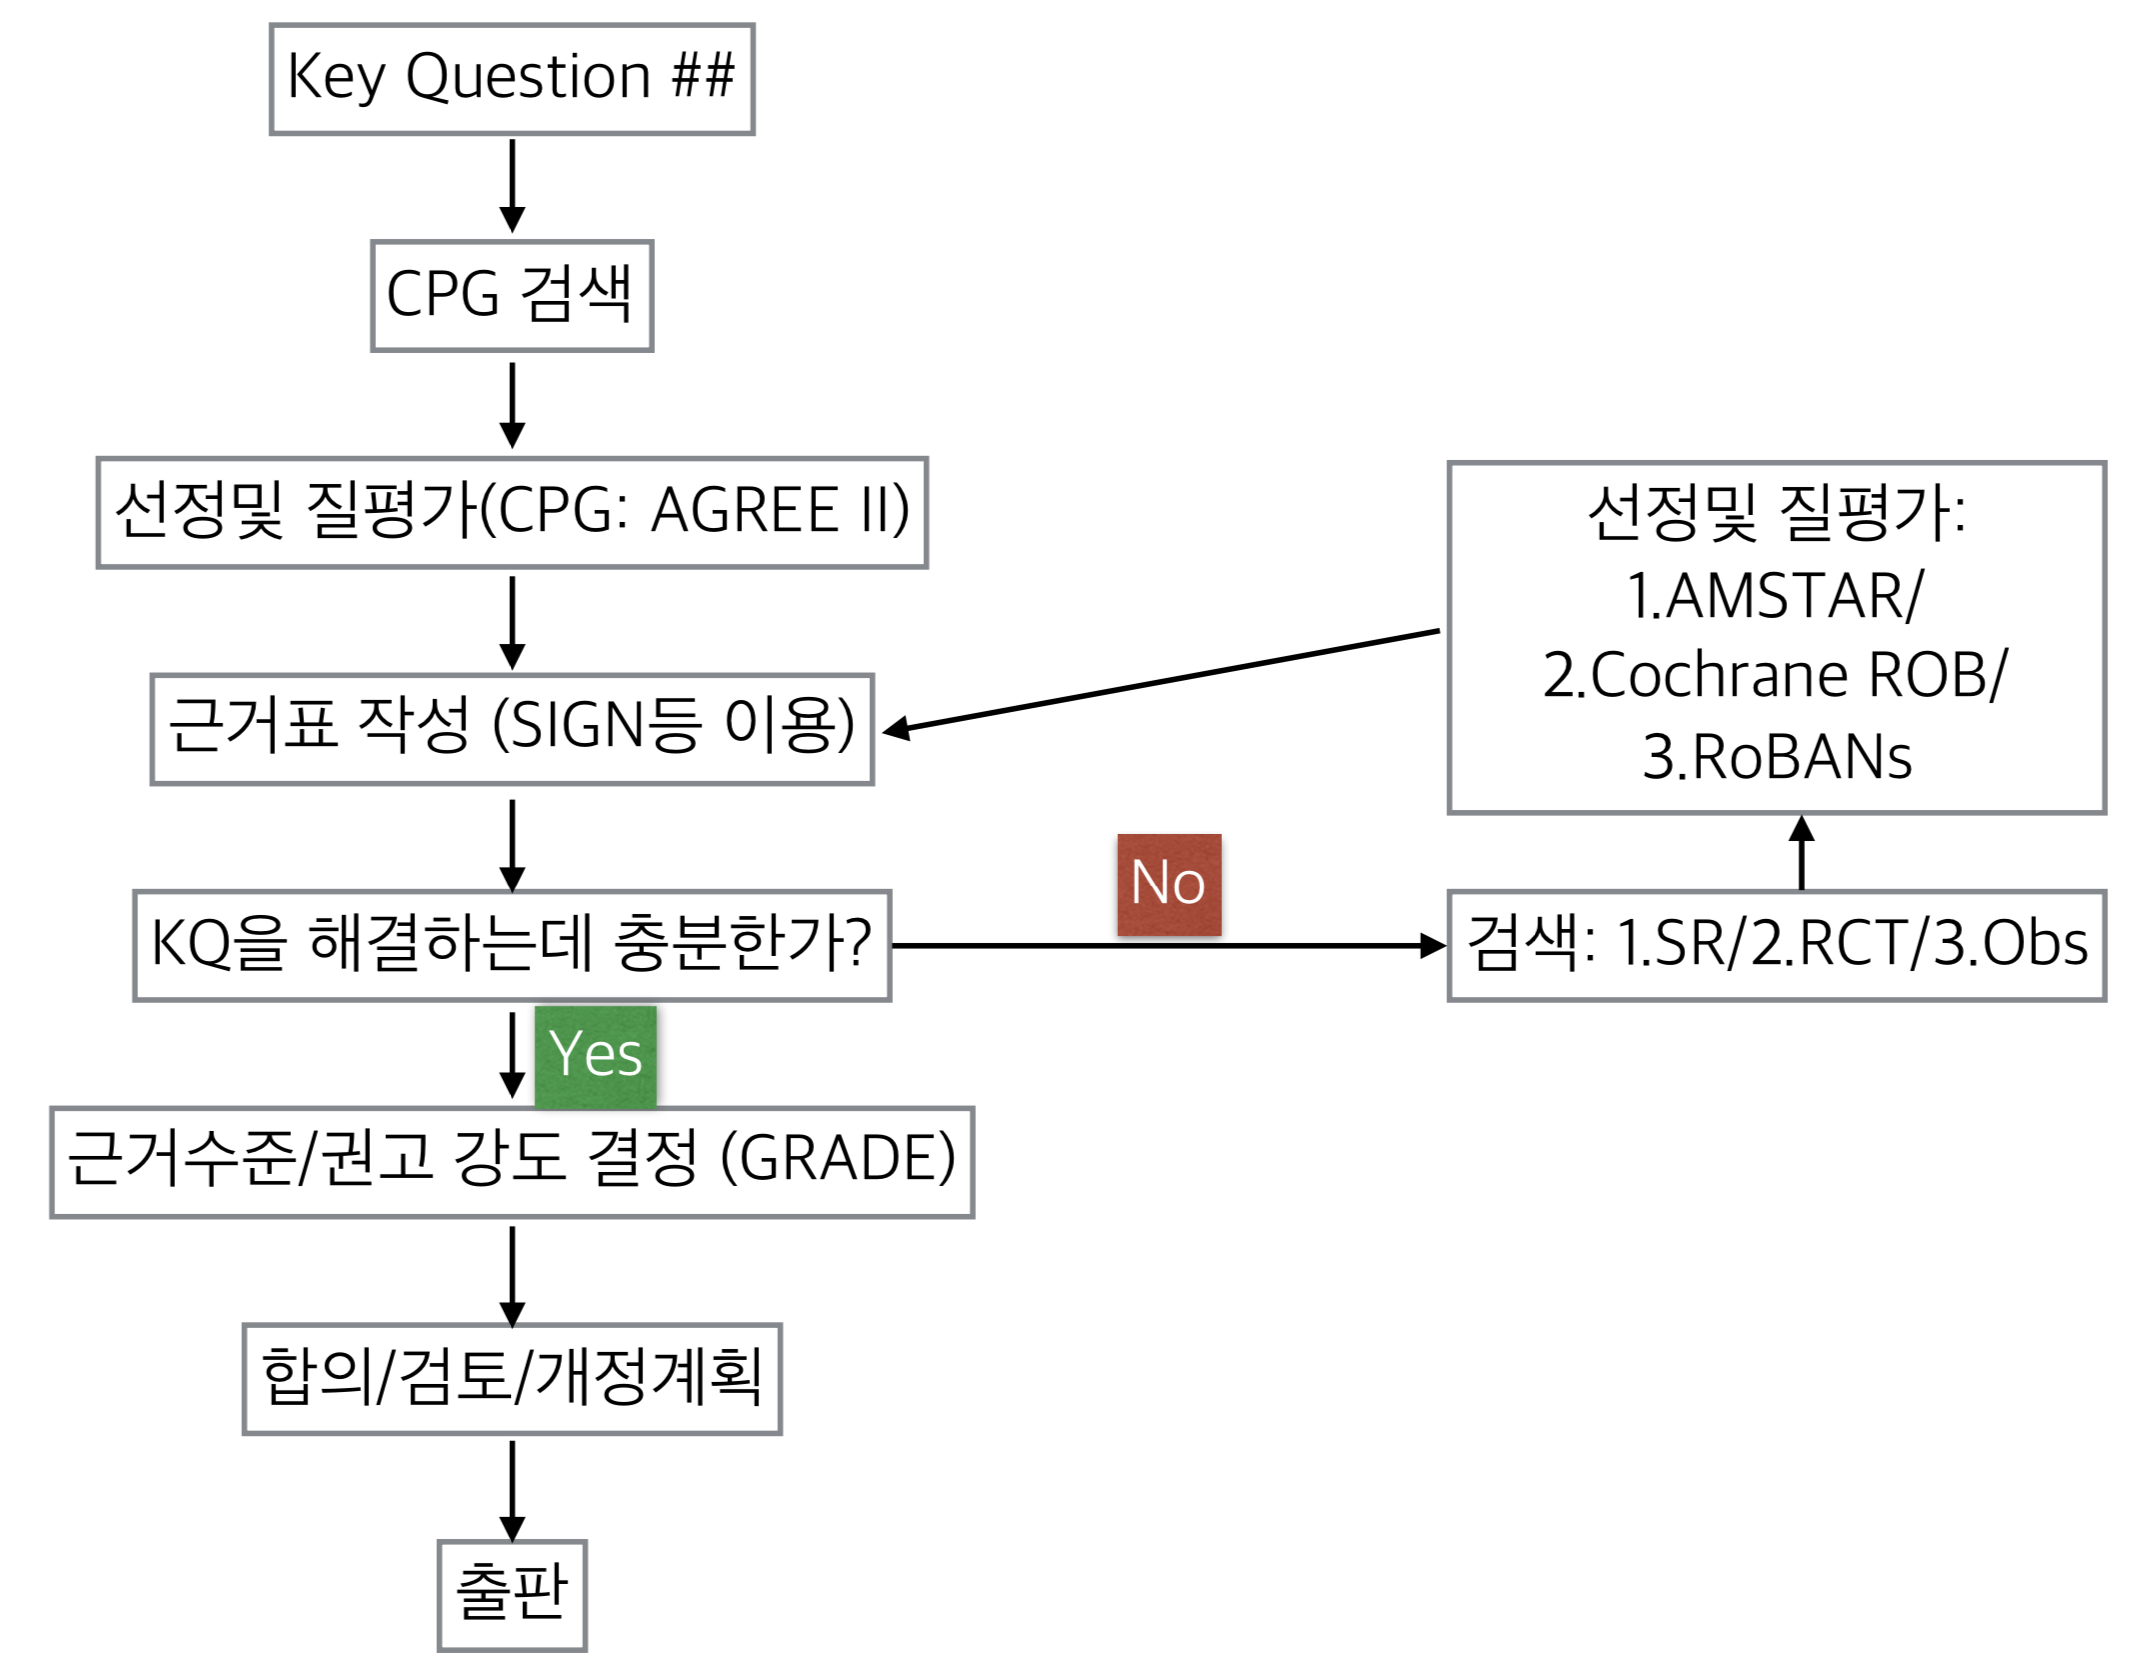
\includegraphics{static/SearchProcess.png}

\bibliography{book.bib,packages.bib}


\end{document}
